\documentclass{../tikz_figure}
\begin{document}
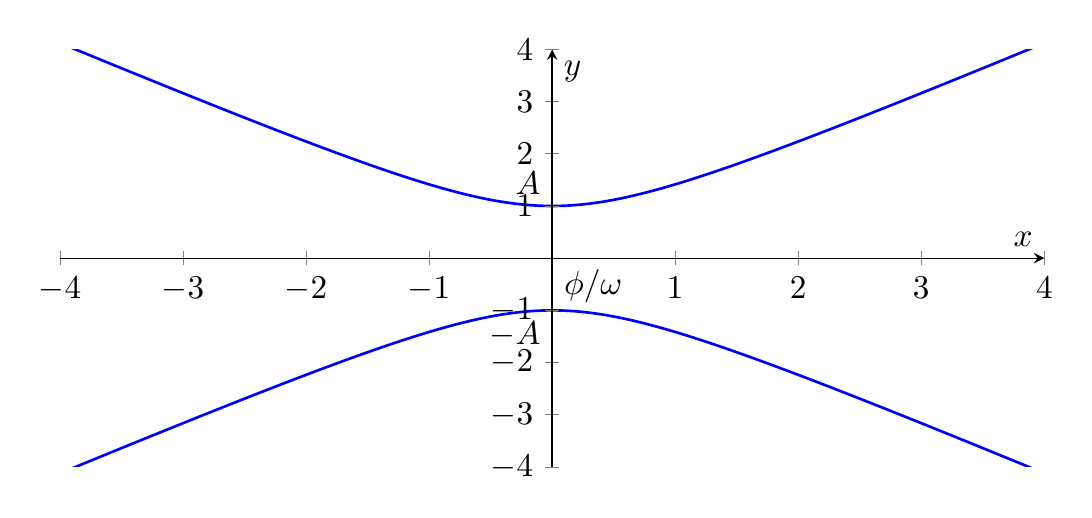
\begin{tikzpicture}[scale=1.2]
	% \clip (-4,-4) rectangle (4,4);
	\begin{axis}[
			axis lines=middle,
			xlabel={$x$},
			ylabel={$y$},
			xmin=-4, xmax=4,
			ymin=-4, ymax=4,
			samples=200,
			grid=none,
			domain=-4:4,
			xtick={-4,-3,...,4},
			ytick={-4,-3,...,4},
			width=12cm,
			height=6cm,
			enlargelimits=false,
			clip=true,
			axis on top,
		]
		% 绘制双曲线
		\addplot[blue, thick] {sqrt(x^2+1)};
		\addplot[blue, thick] {-sqrt(x^2+1)};
		\node[anchor=south east] at (axis cs:0,1) {$A$};
		\node[anchor=north east] at (axis cs:0,-1) {$-A$};
		\node[anchor=north] at (axis cs:pi/6/3.1416/0.5,0) {$\phi/\omega$};
	\end{axis}
\end{tikzpicture}
\end{document}

